\documentclass[11pt]{article}
\usepackage[utf8]{inputenc}
\usepackage[T1]{fontenc}
\usepackage{amsmath}
\usepackage{geometry}
\usepackage{graphicx}
\geometry{margin=2.5cm}

\begin{document}

\begin{center}
{\LARGE\bfseries Validation empirique du Théorème 5}
\end{center}
\vspace{1em}

Le Théorème 5 garantit la récupération exacte de la cible tant que
$\eta < \mu/M$. Pour vérifier ça sans dépendre de $n$, on trace le taux
de succès en fonction de $r = \eta/\eta_{\max}$ (le bruit relatif au
seuil garanti), avec une clause entraînée sur 100 epochs, $N=3\,000$
états par automate, mélangeant $n=4$ à $12$.

\begin{center}
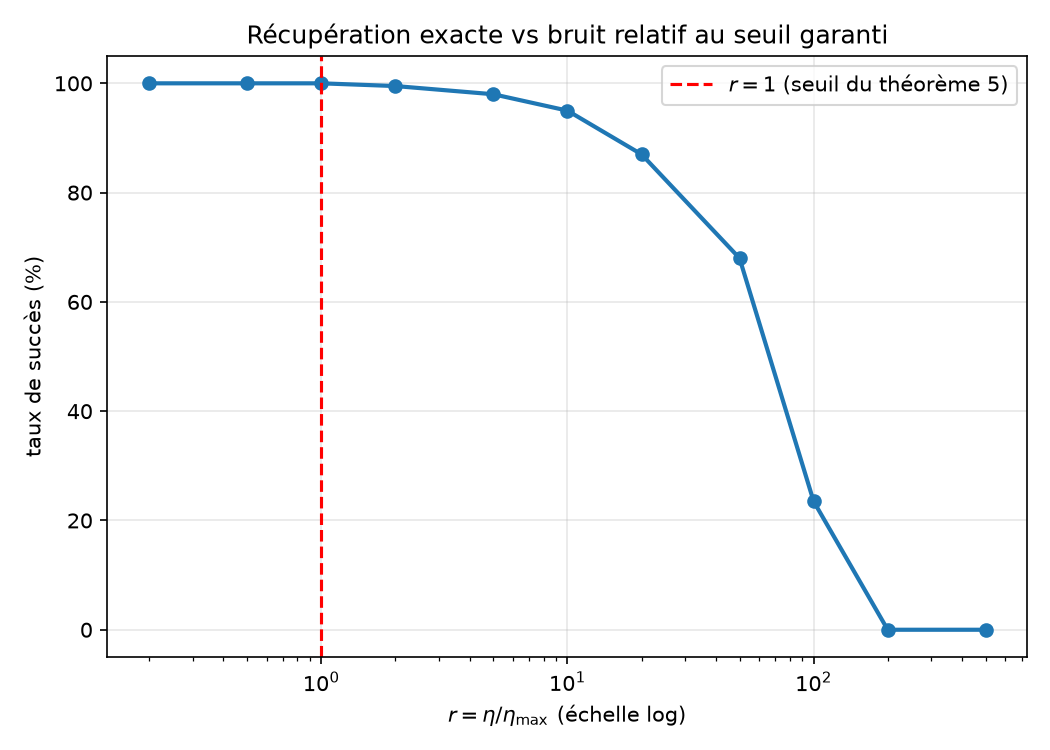
\includegraphics[width=0.85\textwidth]{figures/succes_vs_r_theoreme5.png}
\end{center}

\textbf{Résultat} : 100\% de succès jusqu'à $r=2$, soit bien au-delà du
seuil garanti $r=1$. La dégradation commence vers $r=5$ et s'effondre
entre $r=100$ et $r=200$. Rien n'indique de rupture avant $r=1$ : le
seuil du théorème est confirmé, et la règle tolère en pratique un bruit
nettement supérieur à ce que la borne garantit formellement pour ce
jeu de paramètres.

\end{document}
